\section{Design and Implementation of \textsf{PCStream}}
In this section, we describe in detail the proposed automatic stream management technique,
\textsf{\small PCStream}.  We first explain how we automatically extract PCs during
runtime and describe how multiple PCs are mapped to streams in an SSD.

Fig.~\ref{fig:architecture} shows an overall organization of \textsf{\small PCStream}.
\textit{The PC extractor module}, which is implemented in the Linux kernel as
part of a system call handler, 
computes a PC signature, which is used as a unique ID for each program context.  
We use the signature program counter~\cite{PC} as a PC signature 
by summing program counter values along the execution path to a write-related system function 
(e.g., {\tt write()}).  
With the PC signature, we can monitor the data lifetime of each write at the program context level. 
A PC signature value is stored
in an inode data structure of a file system (modified for \textsf{\small PCStream})
and is delivered to \textit{the lifetime analyzer module} which estimates
expected lifetimes of data belonging to a given PC in the block device level.
In order to efficiently detect the end of data lifetime in append-only
workloads, the lifetime analyzer also intercepts TRIM~\cite{TRIM} requests from a file system.  %shane part
Based on the lifetime information, \textit{the PC-to-stream
mapper module} clusters PCs with similar lifetimes and maps them together to
the same stream ID.  This mapping is required because 
the number of streams in an SSD is generally less than the number of PCs in host applications.

\subsection{Automatic PC computation}
As mentioned earlier, a PC is represented by a PC signature which is defined as
the sum of program counter values along the execution path of a function call that
finally reaches a write-related system function. A function call involves
pushing the next program counter, which is used as a return address, to the
stack followed by pushing a frame pointer value.  In general, by using frame
pointer values, we are able to back-track the stack frames of the process and
selectively get return addresses for generating a PC signature.  For example,
Fig.~\ref{fig:getpc}(a) shows the abstracted execution path for flushing data
in RocksDB and Fig.~\ref{fig:getpc}(b) illustrates how a PC signature is obtained
by back-tracking the stack.  
Since a frame pointer value in the stack holds the address of the previous
frame pointer, the PC extractor can easily obtain return addresses and
accumulate them to compute a PC signature. 
(The return addresses are pushed
before calling the \textsf{\small  write()}, \textsf{\small  BuildTable()} and \textsf{\small 
WriteLevel0Table()} functions.)

\begin{figure}[t]
	\centering
	%\vspace{-10pt}
	%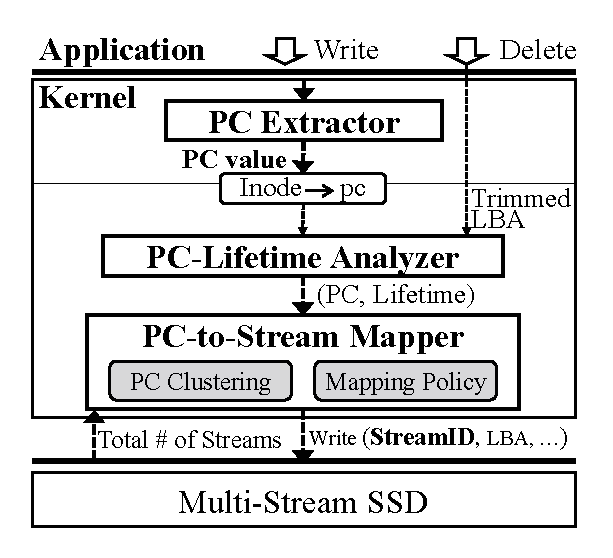
\includegraphics[width=0.6\linewidth]{figure/architecture4}
	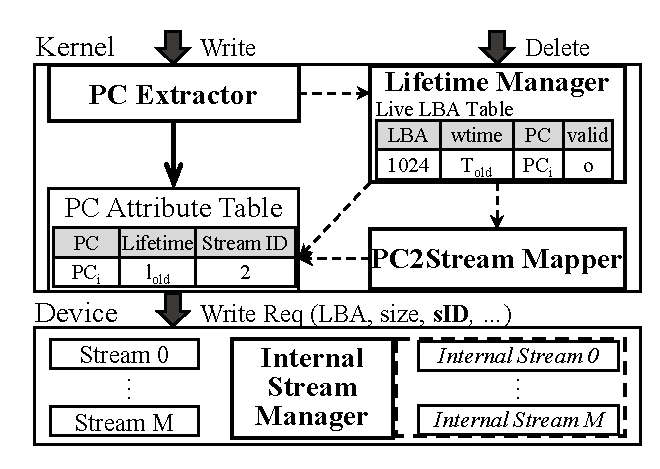
\includegraphics[width=0.6\linewidth]{figure/overview}
	%\vspace{-9pt}
	\caption{An overall architecture of \textsf{\small PCStream}.}
	\label{fig:architecture}
	%\vspace{-22pt}
\end{figure}


The frame pointer-based approach for computing PC signatures, however, is not
always possible because modern C/C++ compilers often do not use the frame
pointer for improving the efficiency of register allocation.
One example is a
{\tt -fomit-frame-pointer} option of GCC~\cite{GCC}. 
Although this option allows the frame pointer to be used as a general-purpose
register for high performance, it makes very difficult for us to back-track
return addresses along the call chains.  

\begin{figure}[b]
%	\vspace{-10pt}
	\centering
	%\vspace{-8pt}
	\subfloat[An abstracted execution path for flushing data.]{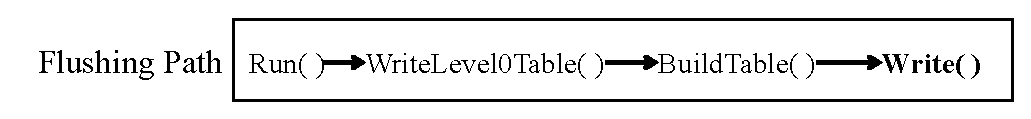
\includegraphics[width=0.4\textwidth]{figure/getpc_1}}  
	%\vspace{-14pt}
	\hfill
	\subfloat[with the frame pointer.]{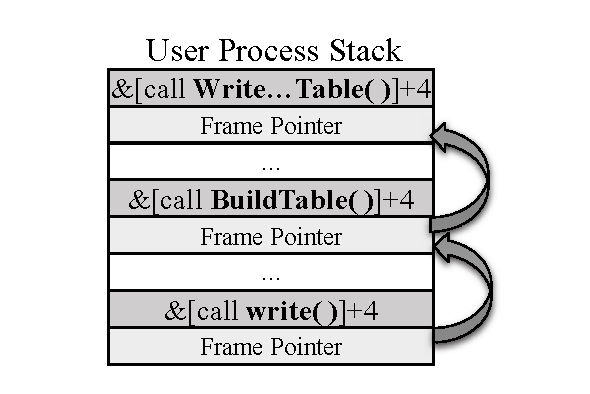
\includegraphics[width=0.22\textwidth]{figure/getpc_2}}
	\subfloat[without the frame pointer.]{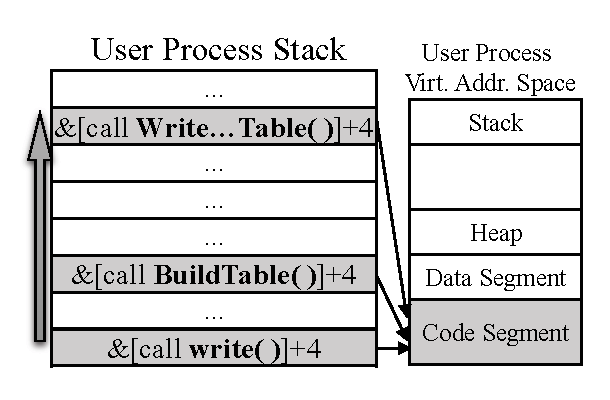
\includegraphics[width=0.22\textwidth]{figure/getpc_3}}
	%\vspace{-9pt}
	%\caption{An example execution path and its PC extraction methods.}
	\caption{An example execution path and its PC extraction.} %shane part
	\label{fig:getpc}
	%\vspace{-20pt}
\end{figure}

In \textsf{\small PCStream}, we employ a simple but effective workaround 
for backtracking the call stack when the frame pointer is not used.
When a write system call is made, we scan every word in the stack and check
if it belongs to the process's code segment.  If the scanned stack word holds a
value within the address range of the code segment, we assume that it is a
return address.  Since scanning the full stack takes too long, we stop the
stack scanning procedure when a sufficient number of return address candidates
are found.  In the current version, we stop when 5 return address candidates
are found.  Although quite ad-hoc, a restricted scan is effective in
distinguishing different PCs because two different PCs
cannot follow the same execution path to write system functions.  
(If they do, they are the same PC.) In our evaluation
with a 3.4 GHz CPU machine, the performance overhead of the restricted scan was
almost negligible, taking only 300-400 $n$sec per write system call.

\subsection{PC extraction for indirect writes}
{\color{blue}추가: write system call을 직접 호출하지 않는 indirect write을 하는 application에 대해서도 확장.
예를 들어, cassandra와 같이 JVM 기반의 응용은 write system call을 직접 호출하는 대신, Java가 제공하는 interface
를 사용하여 간접적으로 쓰기 수행. 이 경우, Java interface를 통해 쓰기 수행 시, PC extractor를 수행하고
얻은 PC 값을 system call에 전달하여 PC를 얻을 수 있음.
즉, 데이터가 만들어진 context를 정확히 파악할 수 있는 계층에서 PC를 계산함.
이와 비슷한 mmap이나 프로그램 내부 buffer를 사용하는 case에 대해서도 위와 비슷한 접근을 할 수 있지만, 
future work으로 남김.}\\

\subsection{PC lifetime management}
The prediction of PC lifetimes is rather complicated. 
{\color{blue}수정: 데이터 lifetime은 쓰기 request가 issue된 때 부터 해당 주소가 다시 write되거나 
TRIM command에 의해 삭제될 때 까지로 정의된다.}
The data lifetime of the append-only workload is defined 
from when a write request is issued until the TRIM command~\cite{TRIM} is issued to 
the corresponding address.
In order to measure the lifetime of data, the lifetime analyzer 
records the write time and PC value for each write request using its LBA.
Upon receiving the TRIM command, the lifetime analyzer can compute the 
lifetime of the corresponding data using the recorded information.
{\color{blue} 추가: lifetime 관리의 부하를 줄이기 위해 최적화를 적용함.
device 전체 LBA 공간에 대해 쓰여진 시간 정보를 유지하는 것은 메모리 부하가 크기 때문에,
몇 MB 단위로 관리함.}
Note that, the
same PC may generate multiple data streams with different lifetimes.
We take the average lifetime as the PC's lifetime.

{\color{blue} 추가: Section 3에서 언급했듯이, PC는 virtual address 기반으로 계산되므로
한 프로그램의 반복적 수행은 동일한 PC가 생성됨.
프로그램의 수행 사이에도 수명 정보를 유지할 수 있도록
발생한 PC와 그 PC의 수명 정보를 caching하는 모듈이 추가됨.}

\subsection{Mapping PCs to SSD streams}

The last step in \textsf{\small PCStream} is to map
a group of PCs with similar lifetimes to an SSD stream.
This is because each SSD supports a limited number of stream IDs. For
example, SSDs used in \textsf{\small FStream}~\cite{FStream} and \textsf{\small AutoStream}~\cite{AutoStream}
support only 9 and 16 streams, respectively. 
{\color{blue} 수정: PC cluster는 k-means 알고리즘을 사용하여 비슷한 수준의 수명을 가진 PC들을 cluster 함.}
To properly group multiple PCs,
the PC-to-stream mapper employs a simple 1-D clustering algorithm. 
In order to cluster PCs with similar lifetimes, the mapper calculates the 
lifetime difference between PCs.
Then, PCs with the smallest lifetime difference are clustered into the same PC group. 
The mapper repeats this clustering step until all the PCs are assigned to their PC groups.
For adapting to changing
workloads, reclustering operations should be regularly performed. Since the
number of PCs created by applications is not limited, the clustering algorithm
must be efficient enough to quickly handle many PCs. 
{\color{blue} 추가: cluster 수행 횟수를 줄이기 위해 관리하는 PC의 list를 만들어 
새로운 PC가 추가되었을 때만 알고리즘을 수행함.}


